\section{Developer Roles}
Today there are game studios with more than a 1000 employees working on a same project for years.
Usually, each developer has one of the following roles \cite{wikiGameDev}:
\begin{itemize}
 \item level/world designer;
 \item game writer/storyline developer;
 \item game artist/content designer;
 \item programmer/system designer;
 \item interface designer.
\end{itemize}
\begin{figure}[h!]
     \begin{center}
      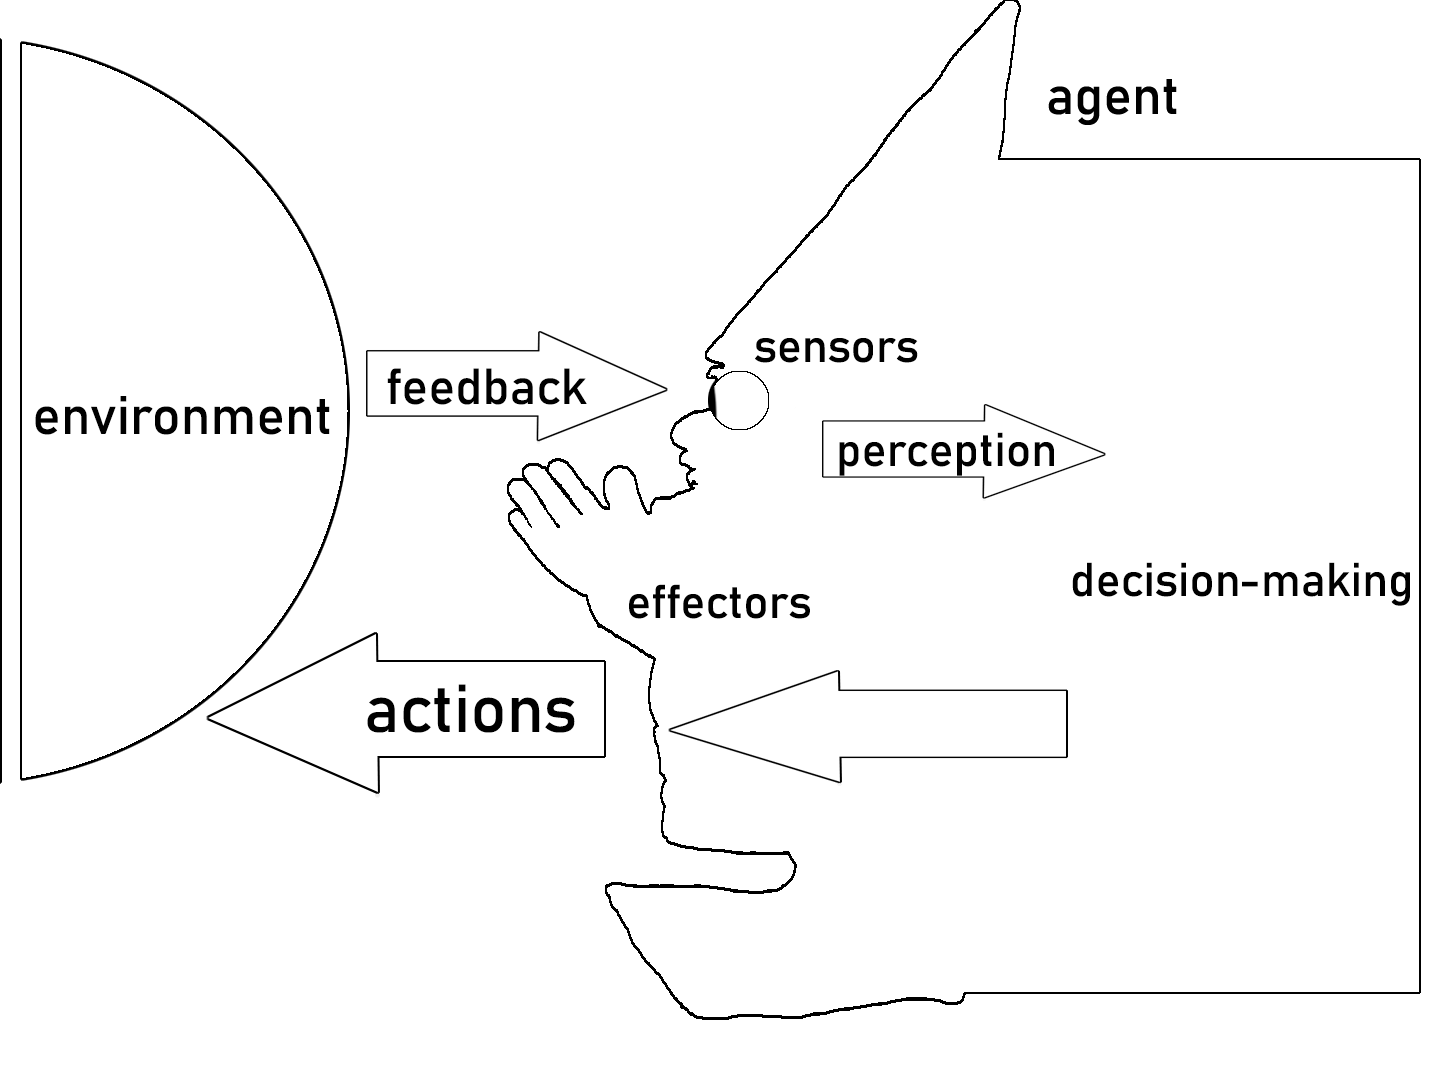
\includegraphics[width=400pt]{gnome_agent}
      \caption{Developer roles}
      \end{center}
\end{figure}
Each role is connected to a specific set of tasks: game artists produce content, level designers and storyline developers assemble the content and connect it to the logical core that is made by programmers, etc. One of the ways to improve overall game development speed is  to partially automate the work of storyline developers.\

The problem lies in deep interconnection of all roles. Storyline developer strongly relies on level designer who usually is unable to work before the content is created. Being unable to communicate with others may result in storyline developer making a story that is impossible to be efficiently implemented within the game. Therefore, the result of storyline designer's work should be understandable for other team members as well as one should take into the account the capabilities of the people one work with. 